%% Springer Nature LaTeX template (sn-jnl.cls, v3.1 December 2024)
%% Reference style: sn-nature (Nature Portfolio journals, including Scientific Reports)
\documentclass[pdflatex,sn-nature]{sn-jnl}

\usepackage{graphicx}%
\usepackage{multirow}%
\usepackage{amsmath,amssymb,amsfonts}%
\usepackage{amsthm}%
\usepackage{mathrsfs}%
\usepackage[title]{appendix}%
\usepackage{xcolor}%
\usepackage{textcomp}%
\usepackage{manyfoot}%
\usepackage{booktabs}%
\usepackage{array}%

%% Editorial placeholders -- REMOVE before submission.
\newcommand{\ednote}[1]{{\color{red!70!black}\small[\textsf{#1}]}}
%% Result numbers are plain in the submitted version.
\newcommand{\num}[1]{#1}

\raggedbottom

\begin{document}

\title[Fourier Phase Space as a Candidate Code for Musical Pitch]{Frequency Range of Fourier Phase Space as a Candidate Code for Musical Pitch Structure: Evidence from
Artificial Neural Network Models of Iranian Classical Music}

\author[1]{\fnm{Yousef} \sur{Aftabi}}\email{yousef.aftabi@uok.ac.ir} 

\author*[1]{\fnm{Hamid} \sur{Farvaresh}}\email{farvaresh@uok.ac.ir} 

\affil[1]{\orgdiv{Department of Psychology}, \orgname{University of Kurdistan},
\orgaddress{\city{Sanandaj}, \country{Iran}}}

\affil*[1]{\orgdiv{Department of Industrial and System Engineering}, \orgname{University of Kurdistan},
\orgaddress{\city{Sanandaj}, \country{Iran}}}


\abstract{How is musical pitch structure represented across cultures? Artificial neural
networks trained on Western tonal classification problems spontaneously develop connection
weights correlated with discrete Fourier phase spaces of the 12-tone pitch-class system. We
test whether this extends to a structurally distinct microtonal system: Iranian classical
music, whose 17 pitch classes lie on a 24-tone quarter-tone lattice and are not a subset or
transposition of the Western chromatic scale. We defined nine classification tasks from
Iranian music theory, covering melodic intervals and Dangs, trained Gaussian value-unit
networks on each, and within the same pipeline trained matched networks on Western 12-tone
tasks. Across every task, hidden units were reliably dominated by a single Fourier phase
space: this exceeded a permutation null under false-discovery-rate control and outperformed
pitch-height and random baselines. Iranian networks recruited the full range their lattice
permits (1--12) and Western networks theirs (1--6). Excluding the Nyquist phase space,
which on a quarter-tone lattice degenerates into a chromatic/microtonal partition, and
matching task type, 31\% of Iranian units occupy frequencies 7--11 that a 12-tone lattice
cannot represent, against none of the Western units. A label-permutation control collapsed
all fits to chance, indicating the structure is task-driven. Fourier phase space is thus a
representational format networks discover beyond Western tonal music.}

\keywords{music cognition, discrete Fourier transform, Iranian classical music, cross-cultural comparison, pitch-class representation}

\maketitle

\section{Introduction}

Music is documented in every known human society, appears to have been present from the
earliest periods of organized human social life, and is plausibly counted among the most
ancient cognitive traits of our species \cite{pearce2012,zatorre2013}. Listening to,
performing, and creating music recruits an unusually broad swath of cognitive machinery,
drawing on auditory perception, attention, memory, expectation, and emotion in concert
\cite{zatorre2005}. A central question for cognitive science is therefore how the human
brain represents this structurally rich, temporally extended, and culturally variable
stimulus class. Despite substantial progress in the cognitive neuroscience and behavioral
study of music, the format of musical representation in the brain remains unresolved
\cite{sankaran2018}, and it is similarly unclear to what extent even basic dimensions of
musical experience, such as the perceived emotional content of a passage, generalize
across listeners from different musical cultures \cite{vuust2022}. Large-scale
comparative work has begun to clarify what is, and is not, shared across musical cultures
at the level of overt behavior. A cross-cultural corpus analysis of ethnographic and
recorded song from a representative sample of the world's societies found that music,
including tonality itself, is present in every society sampled, while also documenting
substantial variation in musical behavior, more within societies than across them
\cite{mehr2019}. Other work fills in the picture. Corpus analyses of folk melody find recurring statistical
regularities in scale construction and interval size across hundreds of societies
\cite{savage2015}. Direct perceptual comparisons between Western listeners and
populations with minimal exposure to Western harmony reveal substantial cross-cultural
variation in judgments of consonance and dissonance \cite{mcdermott2016}. Large surveys
of rhythm perception likewise find a mixture of broadly shared and culture-specific
structure in listeners' mental representations of musical time \cite{jacoby2024}. Partial universality alongside clear
cultural specificity: this is what a satisfying account of musical representation must
explain. A position paper surveying the field has argued explicitly that progress on the
question requires moving beyond the historical reliance on Western participants and
Western musical material \cite{jacoby2020}. This pattern
motivates the search for a representational format that could plausibly support both
shared and culture-specific structure within a single underlying code.

The auditory-neuroscience literature offers a complementary motivation for that search.
Auditory neuroscience has long distinguished place-based and temporal mechanisms of
frequency coding in the peripheral and central auditory system \cite{oxenham2018}, and
intracranial recordings during music listening indicate that distinct, partially
independent neural populations and frequency ranges of ongoing cortical activity carry
functionally separable musical information, from basic pitch height to higher-order
melodic expectation \cite{sankaran2024}. If the human auditory and cognitive system genuinely partitions musical information by
frequency in this way, a representational scheme built explicitly around frequency
components is a natural computational candidate for the format such partitioning might
take. The Discrete Fourier Transform is one such scheme. This holds independently of
whether any particular implementation in artificial neural networks is biologically
realistic.

One comparatively underused strategy for probing musical representation is cognitive
modeling with artificial neural networks (ANNs). Rather than specifying in advance how
musical information ought to be encoded, this approach trains networks to solve
well-defined musical problems and then examines the internal structure that emerges from
training, in order to characterize, post hoc, the representational solutions the network
discovered \cite{dawson2018}. Because nothing in a network's architecture, learning
rule, or training procedure presupposes any particular representational format,
regularities that consistently emerge across independently trained networks constitute
relatively strong evidence that those regularities are well suited to the structure of the
problem itself, rather than artifacts of the modeler's assumptions.

This strategy has only recently begun to be applied cross-culturally.
Matsunaga et al.\ \cite{matsunaga2026} trained deep recurrent neural networks on Western and contemporary
Japanese melodic material to test a bootstrapping account of how culture-specific musical
scales might be learned from exposure alone, and found that a perceptually salient pitch
within each melody could serve as a self-detected training signal for scale acquisition in
both musical cultures. That study, like the present one, uses cross-cultural ANN
simulation to ask whether a single learning mechanism, rather than culture-specific
machinery, can account for how listeners acquire structurally different tonal systems. It
targets the acquisition of scale schemas from melodic sequences. The present study targets
the representational format that emerges once interval and tetrachord categories have
already been learned. The two approaches are complementary tests of the same broader
question about domain-general versus culture-specific musical learning mechanisms.

Over the past two decades, the Discrete Fourier Transform (DFT) of musical structures has
become one of the most productive analytic tools in music theory \cite{harding2021}.
Pitch-class sets, scales, and rhythms can each be treated as periodic functions. Their
Fourier decompositions, and particularly the magnitude and phase of the low-order
components, recover music-theoretically meaningful quantities such as chord quality, key
distance, and macroharmonic structure \cite{amiot2016}. The approach originates in Lewin's \cite{lewin1959} observation that the Fourier transform of a pitch-class distribution captures intervallic
relations between sets of notes, and was substantially formalized by Quinn's \cite{quinn2007} treatment of chord quality. It has since been extended in several directions relevant to
the present work. Yust \cite{yust2015} showed that the phases of low-order Fourier components
define a geometric space, Fourier phase space, closely paralleling the Tonnetz and other
voice-leading geometries. \cite{bernardes2016} constructed a multidimensional Tonal
Interval Space, weighting Fourier components by empirically measured consonance.
Viaccoz et al.\ \cite{viaccoz2022} used DFT-based wavescapes to visualize tonal hierarchy across an
entire musical work. Most recently, Pereira et al.\ \cite{pereira2025} introduced a Fourier qualia space
built from DFT magnitudes to formalize harmonic ambiguity. This continued, active development indicates that the
magnitude and phase information recoverable from the DFT of pitch-class content remains,
nearly two decades after Quinn's original formalization, a productive and still-expanding
framework for capturing music-theoretically meaningful structure, and one argued to sit
unusually close to the way the auditory system itself organizes pitch information
\cite{amiot2016}.

Building on this music-theoretic foundation, Dawson and colleagues showed that ANNs
trained to solve Western tonal music-classification problems spontaneously develop
connection weights that are highly correlated with discrete Fourier phase spaces, without
ever being instructed to use a Fourier-based representation, and proposed that such phase
spaces constitute a plausible neural code for musical cognition
\cite{dawson2020,perez2023}. This research program has since been substantially extended
and consolidated \cite{perez2025}. The finding is not isolated to one architecture or learning algorithm. A closely related
convergence has since been reported in generative models, where the latent space learned by
variational autoencoders trained on tonal corpora shows substantial rank correlation with
DFT-derived phase spaces \cite{rodrigues2024}. Fourier phase space may therefore be a
representation that multiple, architecturally distinct learning systems independently
discover. Separately,
large-scale behavioral work manipulating the spectral (timbral) content of musical tones
has shown that consonance preferences themselves shift substantially with changes to the
harmonic spectrum \cite{marjieh2024}. Together, this body of work motivates treating
Fourier-based, frequency-organized representations as a serious candidate code for musical
cognition, while cautioning against assuming any single frequency-based template is fixed
across listeners or musical systems. Taken together, this is a strong and, in principle, falsifiable claim. If the DFT is
genuinely a privileged candidate code for musical cognition rather than a code specific to
the structure of Western tonal music, it should also characterize the representations that
networks discover when trained on musical entities from an unrelated, independently evolved
musical culture. The present study tests
this prediction directly, using musical problems drawn from Iranian classical music theory.

Iranian classical music offers a particularly informative test case. It is a tradition
with a distinct and internally coherent theoretical system, characterized by extensive
modal variety and melodic subtlety, and among the relatively few musical cultures to have
preserved a continuous, identifiable practice over a long historical period
\cite{farhat1990}. Critically, its pitch material is not a simple transposition or subset
of the Western chromatic scale: Iranian music theory recognizes 17 pitch classes per
octave, including quarter-tone inflections (Koron and Sori) that have no direct equivalent
in 12-tone equal temperament. A musical culture built on a finer-grained, structurally
distinct pitch-class system therefore provides a useful, if necessarily partial, test of
whether Fourier phase-space coding generalizes beyond the specific cardinality and
structure of the Western chromatic scale on which it was originally documented. We note at
the outset that a single additional musical culture cannot establish cross-cultural
generality on its own; rather, it constitutes a first, falsifiable test of whether the
phenomenon replicates outside the system in which it was discovered.

In what follows, we define a set of classification tasks grounded in Iranian music theory,
covering both melodic intervals and Dangs (tetrachords). We then describe the architecture
and training of the ANNs used to solve them, and construct a principled set of Fourier
phase spaces over the Iranian pitch-class lattice, applying the identical construction to a
matched set of Western tasks. We then examine the relationship between network connection
weights and these phase spaces using permutation-based inference, a spectral-concentration
index, and non-Fourier baselines, and we test the frequency range recruited by each
system. This motivates a hypothesis we consider but do not treat as fully established. Different
musical cultures may be distinguished, at a computational and possibly cognitive level, by
different frequency ranges of a shared Fourier-based representational code.

\section{Methods and Materials}

\subsection{Tasks}
Two families of classification problems were used, one built on melodic intervals and one
on Dangs, the principal scale-like tetrachordal units of Iranian classical music. In both
cases the aim was to classify the musical entity into its named category according to
Iranian music theory.

\textbf{Interval tasks.} The stimulus set comprises all 153 unordered pitch-class pairs
drawn from the 17 Iranian pitch classes, that is, the $\binom{17}{2}=136$ two-note
combinations together with the 17 unisons. Because a stimulus is an unordered set (see
\S2.2), the interval is measured in one fixed direction, ascending from the lower-indexed
to the higher-indexed pitch class. The class label is therefore a deterministic function
of the input. Under this labelling the 153 stimuli fall into 24
distinct interval sizes, which constitute the categories of the first task. The second
task uses the identical 153 stimuli but folds each interval together with its inversion
(sizes $c$ and $1200-c$ cents share a label), yielding 13 categories;
Figure~\ref{fig:architecture} shows a representative network trained on this second task,
together with its learned internal structure. We emphasise that
the networks classify unordered pitch-class sets, not directed melodic motions. A
set-based input cannot, and is not asked to, distinguish an ascending interval from its
descending counterpart.

\textbf{Dang tasks.} A Dang is a tetrachordal scale segment spanning a perfect fourth
between its lowest and highest pitch classes, constructed from an ordered combination of
three intervals \cite{alizadeh2008}. Enumerating all such four-note combinations over the
17 pitch classes yields 246 distinct Dangs falling into 36 interval-signature types. Seven
Dang tasks were defined. All share the same classification logic, assigning each Dang to
its named category, but they differ in how dissonant combinations are treated. Task~1 is
the unreduced baseline: all 246 Dangs are retained and every one of the 36 signature types
forms its own category. Tasks~2--7 then apply a graded dissonance manipulation in matched
pairs, each pair defined by a progressively larger dissonance set (Appendix~1). The
\emph{even-numbered} member of each pair retains all 246 stimuli and collapses the
dissonant Dangs into a single shared category, giving 16, 12, and 8 categories for tasks 2,
4, and 6. The \emph{odd-numbered} member instead drops those stimuli from the training set
altogether, leaving 121, 88, and 62 stimuli in 15, 11, and 7 categories for tasks 3, 5,
and 7. This graded
manipulation allowed us to assess whether the phase-space correlations reported below were
specific to a task formulation or held across a family of related problems. Full task
definitions and Iranian nomenclature are provided in Appendix~1.

\textbf{Matched Western tasks.} The Western tasks are constructed by the identical rule,
substituting the 12 pitch classes of 12-tone equal temperament for the 17 Iranian pitch
classes. The stimulus set is therefore all 78 unordered pairs ($\binom{12}{2}=66$
two-note combinations plus 12 unisons), encoded as 12-dimensional binary vectors. The
first Western task classifies these into the 12 distinct interval sizes; the second folds
inversions, yielding 7 categories. Architecture, activation function, learning rule,
learning rate, weight initialisation, stopping criterion, and number of networks are
identical to the Iranian interval tasks (seven hidden units, 25 networks per task), and
the analysis pipeline applied to the resulting weights is the same code path. Because
Iranian classical music has no Western counterpart to the Dang, the Western battery
contains no tetrachord task; \S3.3 therefore reports a task-matched comparison restricted
to the interval tasks, which exist in both systems. Table~\ref{tab:tasks} lists all
eleven tasks.

\begin{figure}[htbp]
\centering
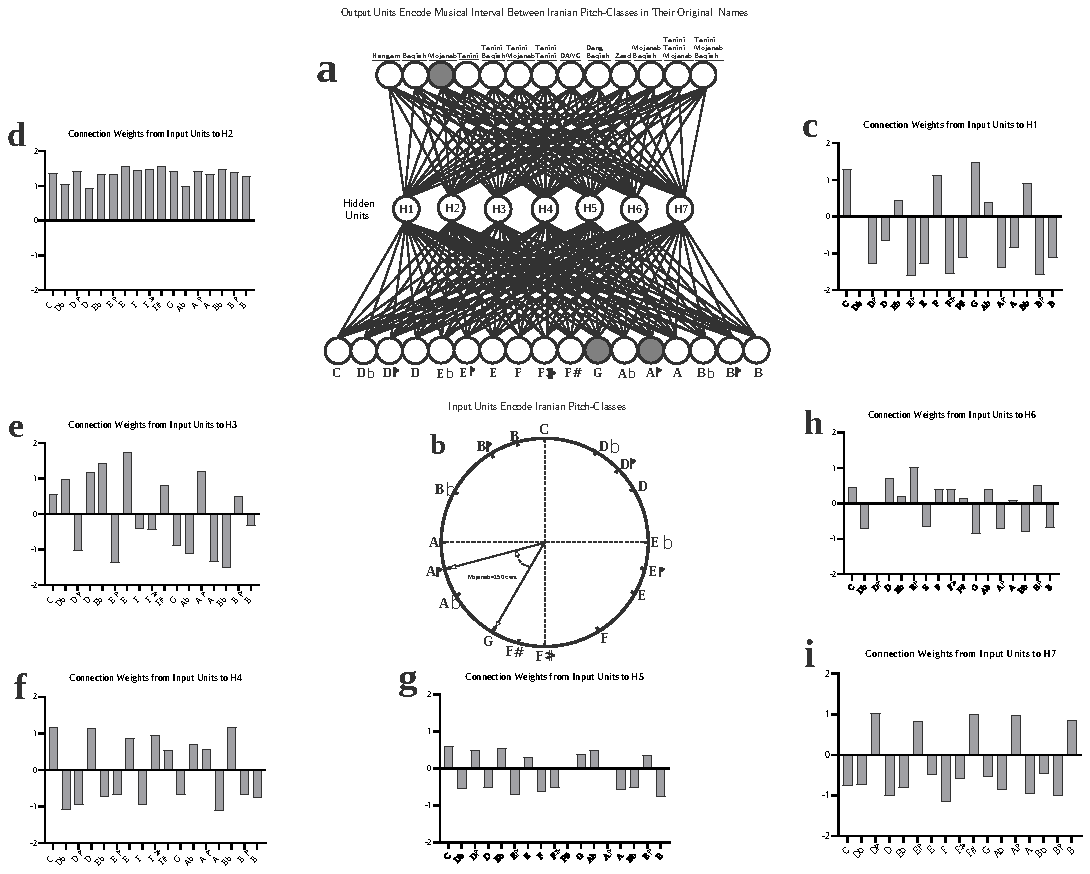
\includegraphics[width=\linewidth]{figures/fig1_architecture.pdf}
\caption{A representative network trained on the second interval task, and its learned
internal structure. \textbf{(a)}~Network architecture: 17 input units (one per Iranian
pitch class), seven hidden units, and 13 output units encoding the named interval
categories that remain once each interval is folded with its inversion.
\textbf{(b)}~The 17 Iranian pitch classes positioned around the octave circle.
\textbf{(c--i)}~Connection weights from the input units to each of the seven hidden units;
each profile is well described by a single Fourier phase space.}
\label{fig:architecture}
\end{figure}

\begin{table}[htbp]
\centering
\caption{The eleven classification tasks. Stimulus and category counts are exactly
reproduced by the analysis pipeline; Western tasks are built by the identical rule on the
12-tone lattice. Dissonance sets A $\subset$ B $\subset$ C are defined in Appendix~1.}
\label{tab:tasks}
\small
\begin{tabular}{@{}llccl@{}}
\toprule
Task & System & Stimuli & Categories & Dissonance handling \\
\midrule
Interval 1 & Iranian-17 & 153 & 24 & --- (inversions distinct) \\
Interval 2 & Iranian-17 & 153 & 13 & --- (inversions folded) \\
Dang 1 & Iranian-17 & 246 & 36 & none; all signature types distinct \\
Dang 2 & Iranian-17 & 246 & 16 & collapse set A \\
Dang 3 & Iranian-17 & 121 & 15 & exclude set A \\
Dang 4 & Iranian-17 & 246 & 12 & collapse set B \\
Dang 5 & Iranian-17 & \phantom{0}88 & 11 & exclude set B \\
Dang 6 & Iranian-17 & 246 & \phantom{0}8 & collapse set C \\
Dang 7 & Iranian-17 & \phantom{0}62 & \phantom{0}7 & exclude set C \\
\midrule
Interval 1 & Western-12 & \phantom{0}78 & 12 & --- (inversions distinct) \\
Interval 2 & Western-12 & \phantom{0}78 & \phantom{0}7 & --- (inversions folded) \\
\bottomrule
\end{tabular}
\end{table}

\subsection{Computational Representation of Musical Stimuli}
Each stimulus was a 17-dimensional binary vector, one dimension per Iranian pitch class (1
present, 0 absent), with a fixed dimension order so that position uniquely identified pitch
class. A Koron sign lowers a pitch by approximately a quarter tone and a Sori sign raises it
by approximately a quarter tone relative to the corresponding natural pitch
\cite{talaei1993}; both inflections were assigned dedicated input dimensions.
Figure~\ref{fig:representation} illustrates the scheme with Dang-e-Shoor, whose four
constituent pitch classes take the value 1 while the remaining thirteen take the value 0.

Critically, the 17 Iranian pitch classes are not 17 arbitrary points on the circle. Under
the modified Vaziri temperament \cite{vaziri1921}, every pitch class falls on a 24-tone
quarter-tone lattice: each position is a multiple of 50 cents ($= 1/24$ octave). The 17
notes occupy 17 of the 24 equally spaced positions:
%
\begin{align*}
\text{lattice indices } g_n &= \{0,\,2,\,3,\,4,\,6,\,7,\,8,\,10,\,12,\,13,\,14,\,16,\,17,\,18,\,20,\,22,\,23\},\\[2pt]
\text{equivalently, cents } &= \{0,\,100,\,150,\,200,\,300,\,350,\,400,\,500,\,600,\\
&\qquad 650,\,700,\,800,\,850,\,900,\,1000,\,1100,\,1150\}.
\end{align*}
%
This lattice structure is what fixes the principled Fourier basis below.

\begin{figure}[htbp]
\centering
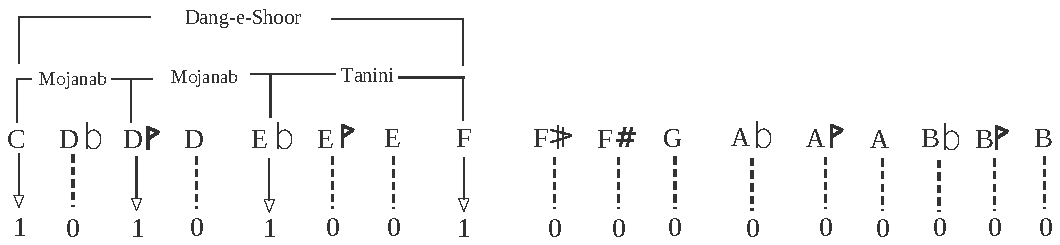
\includegraphics[width=0.92\linewidth]{figures/fig2_computational_representation.pdf}
\caption{Computational representation of a musical stimulus, illustrated with
Dang-e-Shoor. Each stimulus is a 17-dimensional binary vector with one dimension per
Iranian pitch class; a dimension takes the value 1 when its pitch class is present in the
musical entity and 0 otherwise.}
\label{fig:representation}
\end{figure}

\subsection{Architecture of Networks and Training Sets}
Both interval tasks used training sets of 153 stimuli, solved by networks with seven hidden
units. Across the Dang tasks, training-set sizes varied with each task's dissonance-handling
rule (246, 121, 88, or 62 stimuli); hidden-unit counts, set to the smallest value found
sufficient in pilot simulations, were 11, 12, 8, 12, 5, 12, and 4 for Dang tasks 1--7. This
minimal-sufficient choice is standard but not theoretically neutral; we evaluate it directly
with a hidden-layer-size sweep (below).

Networks used a Gaussian (``value unit'') activation function on all hidden and output
units, $a(\mathrm{net}) = \exp(-(\mathrm{net}-\mu)^2)$, with one trainable centre $\mu$ per
unit (initialized to 0), trained with the generalized delta rule and a learning rate of
0.005; connection weights were initialized $\sim\mathcal{U}(-0.1, 0.1)$, and input-pattern
order was re-randomized each epoch. Training continued until every output unit produced a
``hit'' on every pattern (activity $\ge 0.9$ when the target was 1, $\le 0.1$ when the
target was 0). Twenty-five networks were trained per task. The original networks were
constructed in the Rumelhart environment \cite{dawson2008}; for the controls reported
here we re-implemented the identical value-unit network and training rule independently,
and the two implementations agree on the qualitative result. Complete training sets and
trained-network parameters are provided as supplementary materials.

\subsection{Fourier Phase Spaces on the Pitch-Class Lattice}
Yust \cite{yust2016} formalized Fourier phase spaces for Western tonal music by defining six
phase spaces over the 12 Western pitch classes. The pitch classes are positioned around a
circle, and reading the height of each in chromatic order yields discrete samples of a
cosine. The six spaces differ only in the frequency of that cosine, 1 through 6. Because the twelve Western pitch classes are equally spaced (12-TET), this is
exactly the Discrete Fourier Transform of a length-12 signal, whose distinct non-DC
frequencies number $\lfloor 12/2 \rfloor = 6$.

We extend this construction to the Iranian system on its natural lattice. Phase space $k$ is
the two-dimensional span of $\{\cos(2\pi k\,g_n/G),\,\sin(2\pi k\,g_n/G)\}$ evaluated at the
active lattice indices $g_n$, where $G$ is the lattice size, for $k = 1,\dots,\lfloor
G/2\rfloor$. Because the Iranian pitch classes lie on the 24-tone lattice ($G=24$), this
yields \emph{twelve} distinct phase spaces (frequencies 1--12); for the Western 12-tone
lattice ($G=12$) it yields six (1--6). The maximum interpretable frequency is thus set by
the size of the underlying lattice, $\lfloor G/2\rfloor$, and not by the number of active
notes. That is why a quarter-tone system admits phase-space frequencies up to 12 while the
12-tone system admits up to 6. The twelve resulting phase spaces are shown in
Figure~\ref{fig:phasespaces}, each with the circular arrangement of pitch classes at that
frequency and the corresponding cosine samples. This construction reproduces the authors'
original phase-offset procedure exactly: searching a continuous phase offset for the best fit is
equivalent to the two-dimensional cosine/sine projection used here, and for the 12-tone
system the lattice-DFT and the direct construction coincide exactly (an internal validity
check). Because only 17 of 24 lattice points are active in the Iranian system, the
phase-space templates are not perfectly orthogonal over the active points; this
non-orthogonality is precisely why the permutation null and baselines below are required.

\begin{figure}[htbp]
\centering
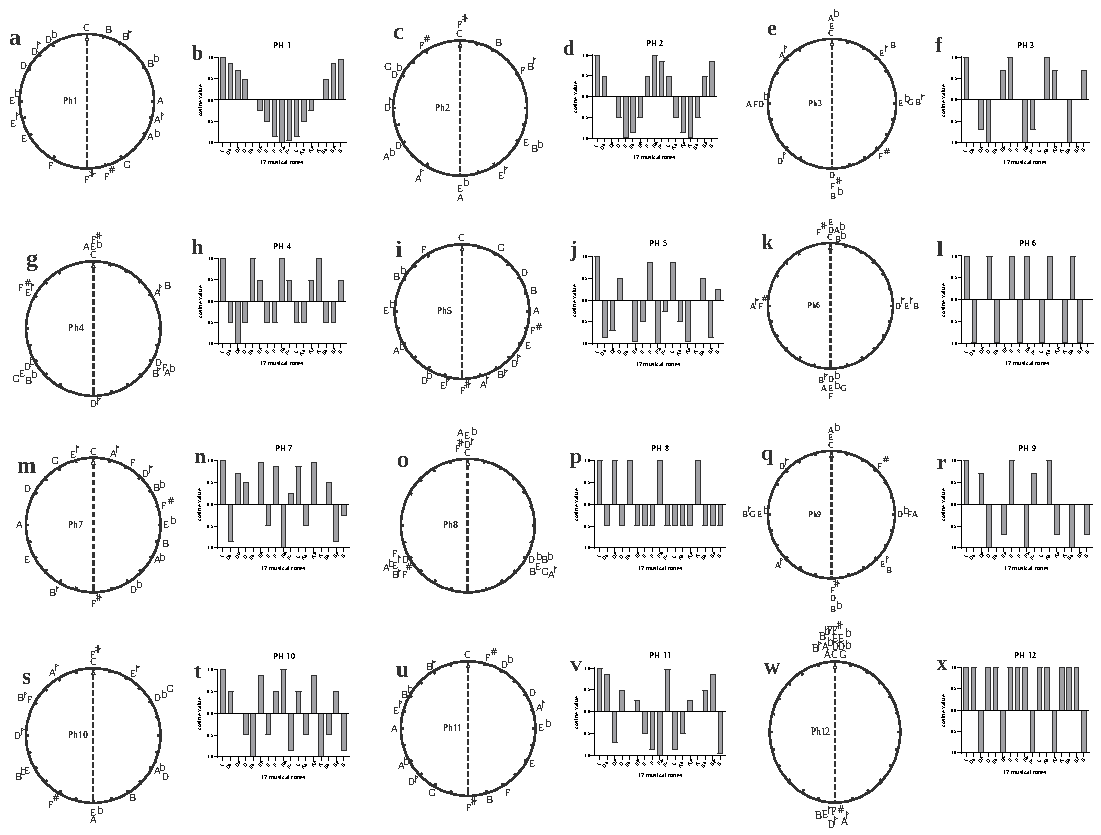
\includegraphics[width=\linewidth]{figures/fig3_phase_spaces.pdf}
\caption{The twelve Fourier phase spaces defined over the Iranian pitch-class lattice.
Each pair of panels shows one phase space: the circular arrangement of the 17 pitch classes
at that frequency (left) and the corresponding cosine samples read around the circle
(right), for frequencies 1 through 12.}
\label{fig:phasespaces}
\end{figure}

\subsection{Analytic Approach and Statistical Considerations}
For every hidden unit we regressed its mean-centred vector of input connection weights on
the two columns of each phase space and took the multiple correlation $R_k$ as the fit; the
best-fitting phase space is $\arg\max_k R_k$, with ties resolved to the lowest frequency so
that aliasing cannot inflate the recruited range. We report three further quantities. (i) A
\emph{spectral-concentration} index, $R_{k^\star}^2/\sum_k R_k^2$, the share of a unit's
total explained spectral power falling in its single best frequency $k^\star$; this measures
single-phase-space dominance directly, since a unit split across two frequencies retains a
high $\max_k R_k$ but a low concentration. Because the number of candidate phase spaces
differs between systems (12 versus 6), concentration is interpreted against a per-system
chance baseline, computed as the mean concentration of random weight vectors evaluated
under that system's own phase bank (Iranian \num{0.254}, Western \num{0.425}), and is not
compared directly across systems. (ii) A \emph{permutation null}: each unit's best fit was
compared against the distribution of best fits obtained when its weights are randomly
permuted (destroying pitch-class order), with Benjamini--Hochberg false-discovery-rate
control across units within each system. (iii) \emph{Non-Fourier baselines}: the fit was
compared with that of a pitch-height ramp and a random low-pass ceiling. For continuity with
prior work we also record the literal Pearson correlation with the cosine column alone.

\textbf{A structural caveat on the Nyquist phase space.} On the 24-tone lattice, phase
space $k=12$ evaluates to $\cos(\pi g_n)=(-1)^{g_n}$, which is $+1$ at every even lattice
index and $-1$ at every odd index, while its sine component vanishes identically. Since the
even indices are exactly the twelve chromatic pitch classes and the odd indices exactly the
five Koron/Sori inflections, phase space 12 is mathematically identical to a binary
chromatic-versus-microtonal indicator, and is one-dimensional rather than a genuine
two-dimensional phase space. Any unit that simply separates chromatic from microtonal inputs
will therefore correlate near-perfectly with it. We accordingly report the high-frequency
band both with and without $k=12$ and treat the band $7$--$11$ as the confound-free claim
(\S3.2).

\textbf{Controls.} Three controls address whether the Fourier structure is genuinely
task-driven. In the \emph{label-permutation} control, networks were retrained on randomly
permuted output labels; persistence of Fourier fits would indicate an artefact of analytic
flexibility rather than a learned solution. In the \emph{input-coordinate} control, the
mapping from pitch classes to input units was randomly permuted before training, so that
adjacency in the input vector no longer tracked adjacency on the pitch-class lattice;
after training, each network's weight vector was mapped back to the canonical pitch-class
order before fitting. This asks whether the Fourier structure depends on the spatial
arrangement of the input units, which the network could exploit as a scaffold, or on
pitch-class identity and task structure. Preserved fits indicate the latter. In the
\emph{task-matched} control (\S3.3), the system comparison is restricted to the interval
tasks, which are defined by the identical rule in both systems, so that lattice cardinality
is not confounded with task type.

\textbf{Level of analysis and effect sizes.} Because hidden units within a network share a
training history and are not independent, all system-level comparisons of fit strength are
made at the network level, with network identity as the unit of replication. For every
non-parametric test we report the test statistic, sample sizes, and a standardised effect
size (rank-biserial correlation for Mann--Whitney and Wilcoxon tests) alongside the
$p$-value; proportions are reported with Wilson 95\% confidence intervals.

\subsection{Reproducibility}
All simulations and analyses were implemented in Python~3.11 using \texttt{numpy}~1.26,
\texttt{scipy}~1.11, \texttt{pandas}~2.1, \texttt{statsmodels}~0.14, and
\texttt{matplotlib}~3.8 with \texttt{seaborn}~0.13. Pseudo-random number generation used
\texttt{numpy.random.default\_rng} with explicit, recorded seeds: networks for task $t$ and
replicate $i$ were initialised with seed $1000 + 100t + i$, and the permutation nulls used
a separate generator seeded at 0. Every random draw is therefore exactly reproducible, covering weight
initialisation, epoch-wise pattern shuffling, label permutation, input-coordinate
permutation, and the permutation null. The complete pipeline, environment
specification, the trained-network outputs, and a test suite that verifies the stimulus and
category counts of all eleven tasks are provided in the public repository
\ednote{https://doi.org/10.5281/zenodo.22686370}

\section{Results}

\subsection{A single phase space dominates each hidden unit, beyond chance}
For every network across all nine Iranian tasks and the matched Western tasks, each hidden
unit's input weights were more strongly related to one of the phase spaces than to the
others (Figures~\ref{fig:unitfits} and~\ref{fig:rankedcorr}). In the original simulations,
mean best-fit correlations were high across tasks (interval tasks $\approx 0.92$--$0.93$;
Dang tasks $\approx 0.75$--$0.85$); the independent re-implementation reported here
reproduces this pattern, and all inferential statistics below are computed from it. Under
FDR-corrected permutation testing, \num{54}\% of Iranian units (\num{1056}/\num{1950}) and \num{74}\% of Western units
(\num{260}/\num{350}) exceeded chance, with mean best-fit $R = \num{0.89}$ and \num{0.95}
respectively. The spectral-concentration index confirmed single-phase-space dominance
directly, and it sat well above its own chance level in both systems (Iranian mean \num{0.545} versus a chance level of \num{0.254}; Western \num{0.905}
versus \num{0.425}; both observed means exceed the 95th percentile of their own chance
distribution).
Concentration is not compared across systems, since the Iranian lattice offers twelve
candidate frequencies to the Western six, which lowers concentration mechanically.

\begin{figure}[htbp]
\centering
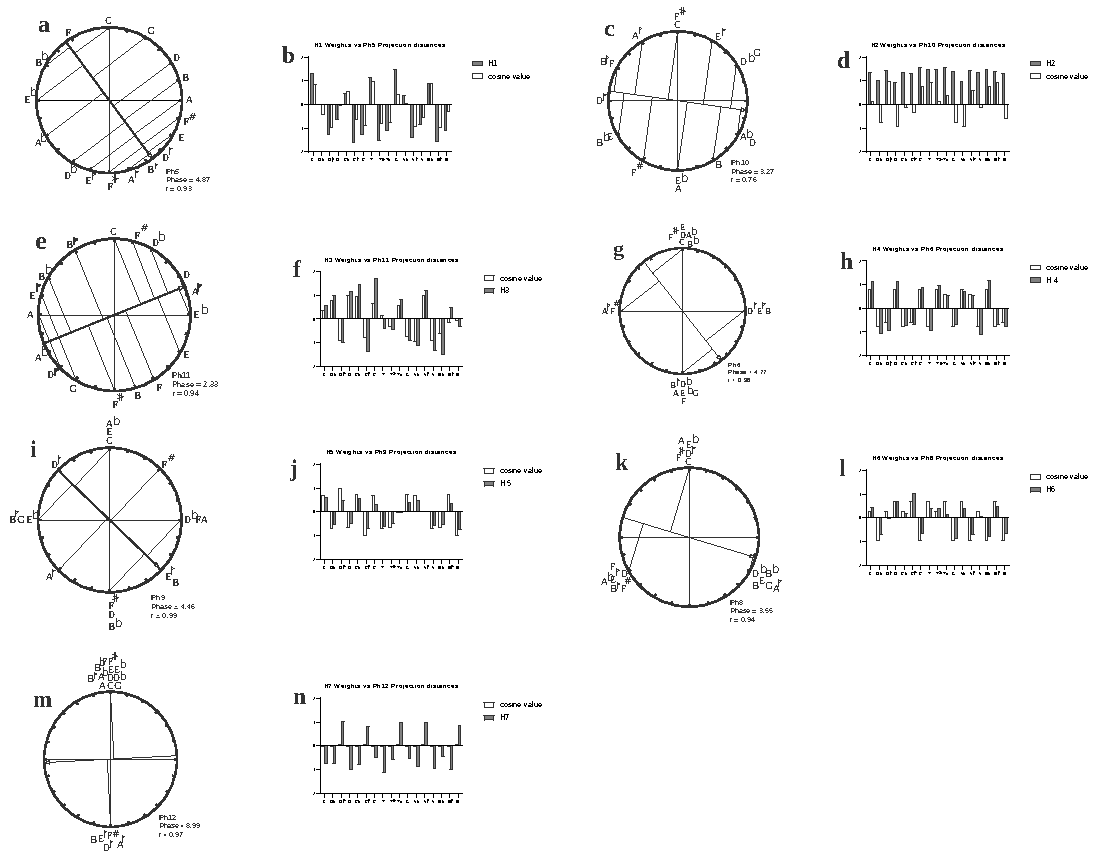
\includegraphics[width=\linewidth]{figures/fig4_unit_fits.pdf}
\caption{Best-fitting phase space for each hidden unit of a representative network. For
each unit, the circular plot (left) shows the phase space to which its weights are most
strongly related, together with the fitted phase and correlation, and the adjacent panel
(right) plots the unit's connection weights against the cosine values of that phase space.}
\label{fig:unitfits}
\end{figure}

\begin{figure}[htbp]
\centering
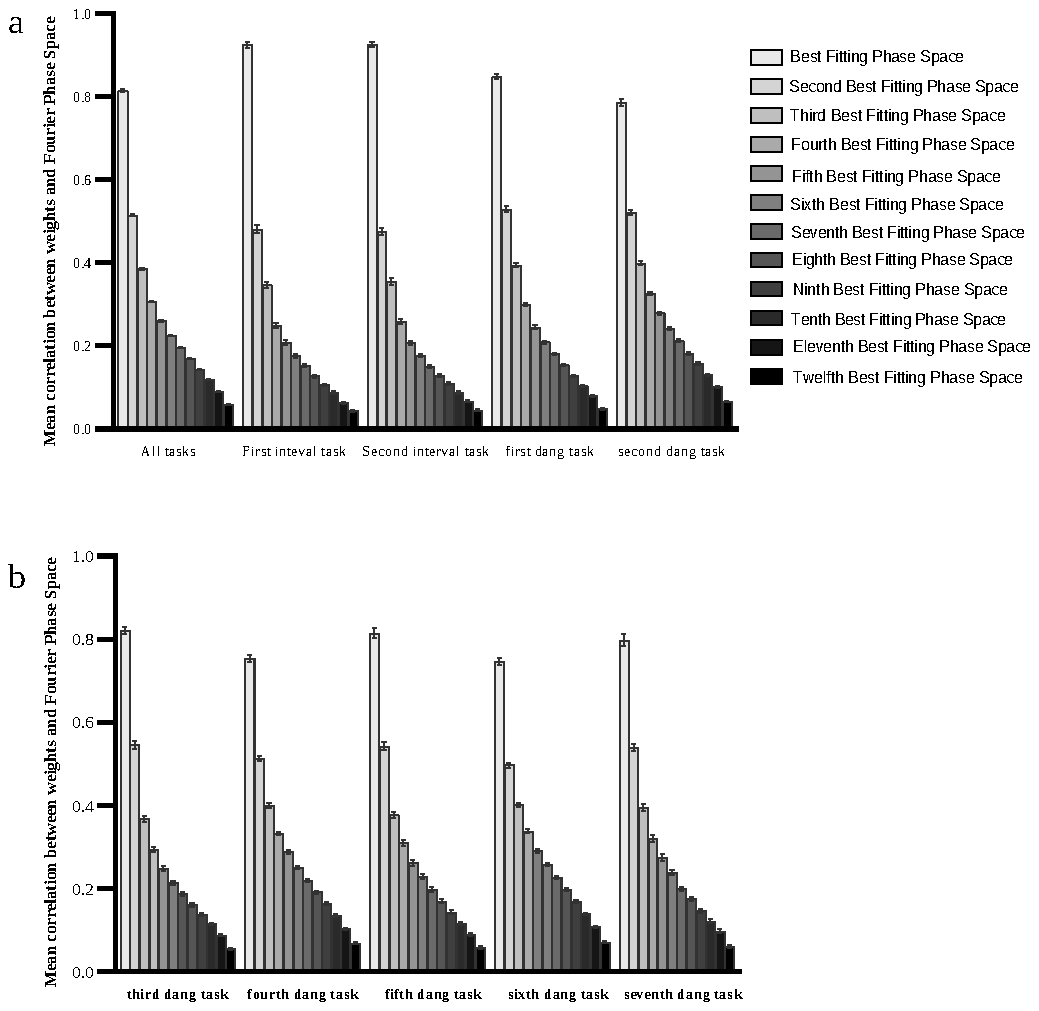
\includegraphics[width=0.94\linewidth]{figures/fig5_correlation_by_task.pdf}
\caption{Mean correlation between hidden-unit connection weights and the Fourier phase
spaces, ranked from the best-fitting to the twelfth best-fitting space, shown separately
for each task. \textbf{(a)}~All tasks pooled, the two interval tasks, and the first two
Dang tasks. \textbf{(b)}~The remaining Dang tasks. In every task the best-fitting phase
space is markedly stronger than the next-best, the pattern quantified by the
spectral-concentration index.}
\label{fig:rankedcorr}
\end{figure}

\subsection{Recruited frequency range, and a construct check on the top frequency}
Iranian significant units spanned every frequency 1--12 and Western units spanned 1--6
(Figure~\ref{fig:freqrange}a,b); both systems reached their lattice Nyquist ceiling. Because
that ceiling scales with lattice size (24 versus 12), part of this difference is guaranteed
on mathematical grounds and is not itself evidence.

Two potential confounds must be removed before the residual difference can be interpreted.
The first is structural. As set out in \S2.6, phase space $k=12$ on the 24-tone lattice is
identical to a binary chromatic-versus-microtonal indicator and is one-dimensional, so units
whose best fit lies there may be simple feature detectors rather than periodic codes. This
matters quantitatively: of the \num{595} Iranian units in the nominal 7--12 band
(\num{56}\% of significant units), \num{339} lie at $k=12$ alone. Excluding the Nyquist
frequency, \num{256} of \num{1056} significant Iranian units (\num{24.2}\%, Wilson 95\% CI
\num{21.8}--\num{26.9}\%) have their best fit in the band 7--11. No Western unit
does, and none could: a 12-tone lattice cannot represent that band at any frequency
(Fisher's exact test, $p < \num{10^{-27}}$). We therefore take the band
7--11, not 7--12, as the confound-free statement of the result.

\begin{figure}[htbp]
\centering
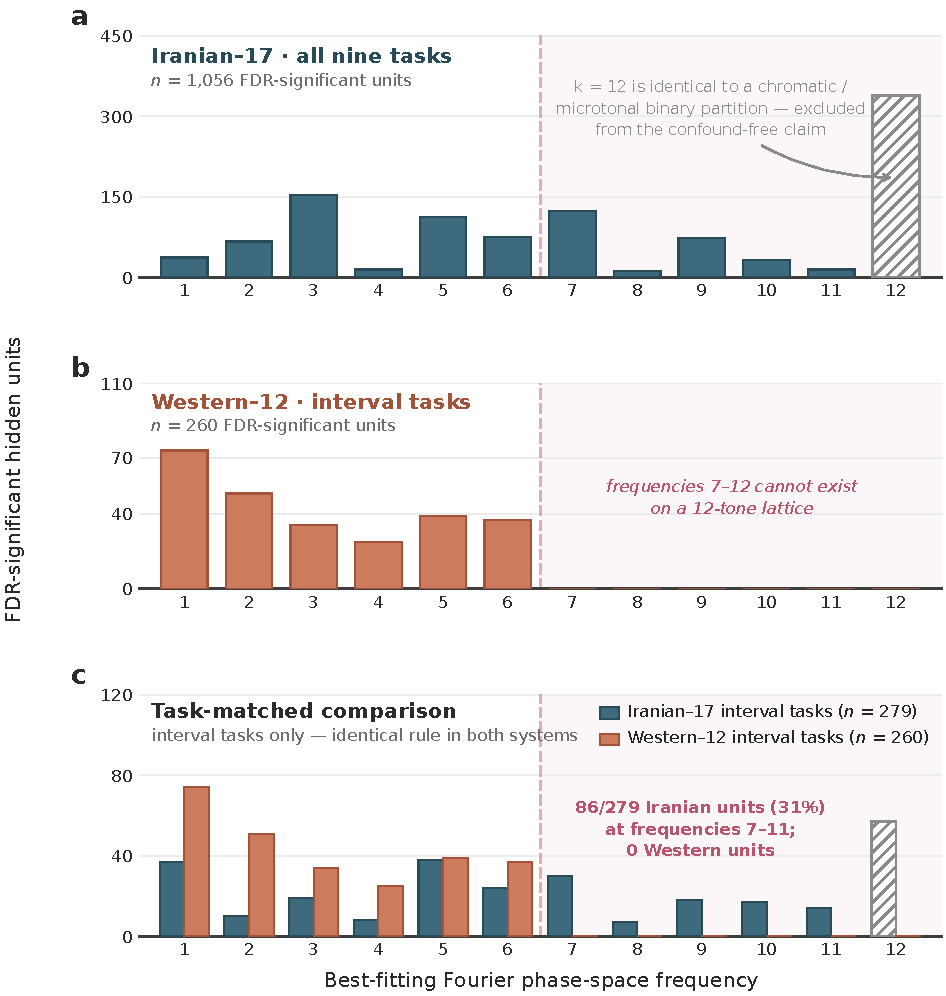
\includegraphics[width=0.94\linewidth]{figures/fig6_frequency_range.pdf}
\caption{Recruited Fourier phase-space frequency. Bars count FDR-significant hidden units
whose best-fitting phase space lies at each frequency. \textbf{(a)}~Iranian-17 networks
across all nine tasks recruit the full range 1--12 permitted by the 24-tone lattice; the
hatched bar at $k=12$ marks the Nyquist phase space, which on this lattice is identical to
a chromatic/microtonal binary partition and is therefore excluded from the confound-free
claim. \textbf{(b)}~Western-12 networks recruit their full range 1--6; the shaded region
cannot be represented on a 12-tone lattice at all. \textbf{(c)}~Task-matched comparison
using only the interval tasks, which are defined by the identical rule in both systems:
\num{86} of \num{279} Iranian interval units (\num{30.8}\%) occupy frequencies 7--11,
against none of the \num{260} Western interval units.}
\label{fig:freqrange}
\end{figure}

\subsection{A task-matched comparison isolates lattice cardinality}
The second confound is task type. The Iranian battery contains seven Dang tasks with no
Western counterpart, so \num{73}\% of Iranian units come from tetrachord problems that have
no analogue in the Western set; tetrachords involve three successive intervals rather than
one, and might plausibly demand higher-frequency structure for reasons unrelated to lattice
cardinality. We therefore repeated the comparison using only the two interval tasks, which
are generated by the identical rule in both systems and differ solely in the underlying
lattice (Table~\ref{tab:tasks}).

The result is unchanged and, if anything, stronger: \num{86} of \num{279} significant
Iranian interval units (\num{30.8}\%, Wilson 95\% CI \num{25.7}--\num{36.5}\%) have their
best fit at frequencies 7--11, against \num{0} of \num{260} Western interval units
(upper bound of the Western Wilson interval \num{1.5}\%; Fisher's exact test,
$p = \num{1.5\times10^{-28}}$; Figure~\ref{fig:freqrange}c). Within
the Iranian system, interval units in fact occupy the 7--11 band \emph{more} often than Dang
units (\num{86}/\num{279}, \num{30.8}\%, versus \num{170}/\num{777}, \num{21.9}\%). The
high-frequency recruitment is therefore not carried by the tetrachord tasks. What the Dang
tasks contribute disproportionately is the confounded $k=12$ peak (\num{282}/\num{777},
\num{36.3}\%, versus \num{57}/\num{279}, \num{20.4}\% for interval tasks), which we have
already excluded. Task type does shift the best-frequency distribution overall
(Mann--Whitney $U = \num{94042}$, $Z = \num{-3.28}$, $p = \num{8.0\times10^{-4}}$,
rank-biserial $r_{\mathrm{rb}} = \num{+0.132}$), but in the direction opposite to the
confound the matched comparison was designed to exclude.

We note one consequence of this scrutiny. In a pooled analysis the \emph{normalised} best
frequency (best frequency divided by each system's Nyquist ceiling) is higher for the
Iranian system (\num{0.635} versus \num{0.490}; network-level Mann--Whitney
$U = \num{9140.5}$, $p = \num{4.7\times10^{-12}}$). That comparison, however, includes
$k=12$, and in the task-matched interval-only analysis the difference is carried almost
entirely by it. With the Nyquist frequency excluded, normalised best frequency does not
differ reliably between the two systems (Iranian \num{0.462}, $n=\num{222}$; Western
\num{0.510}, $n=\num{260}$; Mann--Whitney $U = \num{26594}$, $Z = \num{-1.49}$,
$p = \num{0.14}$, $r_{\mathrm{rb}} = \num{+0.079}$, 95\% CI
$[\num{-0.029}, \num{+0.174}]$).
We therefore do not claim that the Iranian system uses a proportionally higher share of its
range. The claim we do make is categorical rather than proportional: Iranian networks
populate frequencies that a 12-tone lattice cannot express, and they do so at a substantial
rate, while Western networks populate none.

\subsection{The Fourier structure is task-driven}
Retraining on random labels collapsed fit strength. Network-level mean logit-$R$ fell from
\num{1.635} to \num{0.435} in the Iranian networks, a mean paired difference of
\num{1.200} (95\% CI \num{1.124}--\num{1.279}; $n = \num{225}$ networks; Wilcoxon
signed-rank $W = \num{0}$, $r_{\mathrm{rb}} = \num{1.00}$,
$p = \num{1.2\times10^{-38}}$), and from \num{2.814} to \num{0.665} in the Western
networks, a mean difference of \num{2.149} (95\% CI \num{1.910}--\num{2.406};
$n = \num{50}$; $W = \num{0}$, $r_{\mathrm{rb}} = \num{1.00}$,
$p = \num{1.8\times10^{-15}}$). A rank-biserial correlation of \num{1.00} with $W = 0$
means the effect held without exception: every one of the \num{275} networks fitted its
own real-task weights better than its label-shuffled counterpart. The FDR-significant
fraction fell from \num{54}\% and \num{74}\% to exactly zero in both systems.

Permuting the pitch-class-to-input assignment before training, then mapping the learned
weights back to the canonical pitch-class order, left fits essentially unchanged
(mean best $R$ \num{0.775} versus \num{0.779} Iranian; \num{0.891} versus \num{0.906}
Western). This is the expected direction: it shows that the Fourier structure is tied to
pitch-class identity and task structure rather than to adjacency among input units, which
the network cannot have used as a scaffold when that adjacency was scrambled. Together with
the label-permutation result, this indicates that Fourier structure is a solution the
networks discover because of the musical task, not a by-product of the input coding or of
the flexibility of fitting twelve templates to a short weight vector. These were the two
accounts the earlier design could not rule out.

\subsection{Fourier fit exceeds non-Fourier baselines}
The Fourier best fit far exceeded both the pitch-height baseline (\num{0.16} Iranian,
\num{0.24} Western) and the random low-pass ceiling (\num{0.48}, \num{0.57}) in both systems
(all Wilcoxon $p < 10^{-50}$), so a high phase-space correlation reflects specifically
Fourier structure rather than any smooth low-dimensional pattern.

\subsection{Robustness}
Phase-space dominance persisted across a hidden-layer-size sweep spanning deliberately
over-parameterised layers, indicating that the result is not an artefact of the
minimal-sufficient sizing used for the main simulations. As an internal validity check, on
the 12-tone lattice the lattice-DFT construction and the direct construction of Yust \cite{yust2016} coincide exactly.

\section{Discussion}

Across every network trained in this study, the connection weights linking hidden units to
input units were, on average, more strongly correlated with a single Fourier phase space
than with the others. This extends, for the first time, the central finding previously
reported for Western tonal music \cite{dawson2020} to a musical culture whose pitch-class
system is structurally distinct from the Western chromatic scale. Unlike the original report,
the present study establishes this with a matched within-study Western replication, a
permutation null under FDR control, non-Fourier baselines, and a label-permutation control,
so the regularity can now be attributed to the musical task rather than to the analysis.

At no point in a network's training objective, error signal, or learning rule was any
reference made to the Discrete Fourier Transform. Networks were trained only to minimize
classification error on category labels. The label-permutation control sharpens this
observation into a causal one: when the same networks were trained on random labels, the
Fourier fits collapsed to chance. Fourier phase space is therefore a discovered solution
that depends on the structure of the musical task, not merely on the circular input coding
or on the flexibility of fitting twelve templates to a short weight vector. The earlier
design could exclude neither.

Despite substantial surface differences between Iranian and Western musical objects,
networks trained on both cultures converge on a broadly similar representational format,
namely a small number of Fourier phase spaces, each a good descriptor of a hidden unit's
encoding.
The two sets of networks differ most clearly in which frequencies of that code are
recruited across the population of units. Iranian networks recruited the full range 1--12
and Western networks the full range 1--6. Part of this difference is mechanical. The number
of distinct Fourier frequencies is $\lfloor G/2\rfloor$ for a lattice of $G$ steps, so the
higher-cardinality (finer) lattice necessarily admits more frequencies. What is \emph{not}
mechanical is that the Iranian networks actually recruited the higher band, and this
survives the two checks that could most easily have explained it away. Set aside the Nyquist phase space $k=12$, which on a
quarter-tone lattice degenerates into a chromatic/microtonal binary partition and so
cannot count as evidence of periodic coding. Restrict the comparison to the interval tasks
both systems share. On those terms, \num{31}\% of Iranian units still have their best fit
at frequencies 7--11, and none of the Western units do. The networks could have confined themselves to 1--6, as would be the
case were only low-frequency structure useful, but did not. We are correspondingly careful
about what this does \emph{not} show: once $k=12$ is removed, the two systems use
statistically indistinguishable \emph{proportions} of their available ranges, so the
finding is about which frequencies are reachable and populated, not about a shifted
distribution within a normalised range. Independent psychoacoustic work
gives reason to think frequency range carries perceptual weight on its own. Register shapes
perceived consonance even when interval structure is held constant \cite{eerola2022}, and
harmonic consonance depends on the spectral content of a stimulus rather than interval
identity alone \cite{marjieh2024}.

These findings motivate a hypothesis we regard as worth pursuing but not yet established:
that musical cultures might be characterized not by qualitatively different representational
codes, but by different effective frequency ranges of a single, shared Fourier-based code,
tracking properties of the underlying pitch-class lattice such as its cardinality. Such an account would pair shared low-level constraints
on what is representable with culture-specific weighting of which frequencies carry the
distinctions a given system requires. It sits comfortably alongside existing cross-cultural
findings: global musical structure is only weakly related to linguistic or genetic history
\cite{passmore2024}, and the predictive power of psychoacoustic factors for perceived
harmonic tension varies with culture and expertise \cite{armitage2023}.

Testing this hypothesis properly requires musical systems that are genuinely independent of
the one studied here, and this constrains the candidates more sharply than lattice size
alone would suggest. The Arabic and Turkish traditions are the obvious neighbours, but they
are not independent: the Arabic and Turkish maqam systems and the Persian dastgah share a
common historical root, many maqam names are Persian in origin, and the systems influenced
one another throughout their formative period \cite{touma1996}. A confirmation drawn from
them would therefore be a test within one musical family rather than across families, and
would not establish the generality the hypothesis claims. Their theoretical models are also
contested in ways that would force us to choose among competing idealisations: 24-TET is
explicitly a notational convention that does not fix performed microtonal detail
\cite{touma1996}, and the 53-comma Arel--Ezgi--Uzdilek model is standard in theory but only
partially realised in practice \cite{bozkurt2009}. Any ceiling we derived would be an
artefact of that choice rather than a finding.

The informative tests lie further afield, in traditions with independent theoretical
lineages such as the Indian and Chinese classical systems. We deliberately refrain from
stating numerical predictions for them here. Doing so responsibly would require a
well-attested, quantitative specification of the pitch-class lattice each tradition actually
uses, established from within its own theory rather than imposed from outside, and we do not
have that. What the present results do supply is a precise, testable mechanism. Recruited
frequency range should be bounded by the Nyquist frequency of whatever pitch-class lattice a
system employs. Any tradition for which such a lattice can be specified on independent
musicological grounds provides a test, and a system that failed to reach its own ceiling, or
that reached beyond it, would count against the hypothesis.

We should also be explicit about a limitation of our own case. The Iranian simulation rests
on a theoretical idealisation: the modified Vaziri temperament is a twentieth-century
systematisation, and performed Persian music uses flexible, context-dependent intonation
that it does not fully capture \cite{farhat1990}. Our claims concern a well-defined
pitch-class system with a determinate cardinality, and the result depends only on that
determinacy, not on whether the system is an accurate model of performance practice. What
distinguishes this case is that the specification was fixed independently of us. It is the
system in which the networks were originally trained and their stimuli generated, so the
lattice is given by the experiment rather than chosen by the analyst. We record the caveat
in the limitations below: what we have modelled is the Vaziri-theoretic system, not Persian
performance practice.

Finally, an interpretive boundary: these are artificial neural networks trained on idealized,
symbolically encoded stimuli, not models of human listeners, and nothing here licenses a
direct inference from network behavior to human cognitive or neural representation. The
contribution is computational: a precise, reproducible regularity in how a class of learning
systems solves a family of musical classification problems. We offer it as a hypothesis for
future biological work, not as a substitute for it.

\subsection{Limitations}
Several limitations remain, and we state them in the order in which we think they most
constrain the conclusions.

\textbf{The Iranian system is modelled in its theoretical, not its performed, form.} The
modified Vaziri temperament places all 17 pitch classes on an exact quarter-tone lattice;
performed Persian music uses flexible, context-dependent intonation that departs from any
equal division \cite{farhat1990}. Our claims concern a well-specified pitch-class system
with a determinate cardinality and should not be read as claims about performance practice.
A worthwhile extension would perturb the lattice toward measured intonation and ask how
quickly the phase-space structure degrades.

\textbf{The top frequency is not interpretable as periodic coding.} On a 24-tone lattice the
Nyquist phase space coincides exactly with a chromatic/microtonal binary partition, so units
at $k=12$, a third of all significant Iranian units, cannot be distinguished from simple
binary feature detectors. We have excluded them from the central claim, but their prevalence
is itself informative. It suggests that a salient part of what these networks learn about
Iranian pitch material is precisely the chromatic/microtonal distinction. Disentangling this
from genuinely periodic coding at high frequencies would require a lattice on which the two
do not coincide.

\textbf{The task batteries are not fully matched.} Iranian classical music has no Western
counterpart to the Dang, so the Western battery contains only interval tasks. We address
this with a task-matched comparison restricted to the interval tasks, and the result holds
there; but a fuller design would include Western tetrachord tasks constructed by an
analogous rule, allowing the tetrachord manipulation itself to be compared across systems.

\textbf{Two musical systems cannot establish cross-cultural generality.} Genuine generality
requires systems that vary in lattice cardinality, tuning logic, and theoretical structure
independently \cite{jacoby2020}. The neighbouring Arabic and Turkish traditions do not
meet that requirement: they share a historical root with the Persian system rather than
constituting independent cases. Traditions with separate theoretical lineages, such as the
Indian and Chinese classical systems, would be informative, but testing them responsibly
requires a well-attested quantitative specification of the pitch-class lattice each actually
uses, established from within its own theory. We have scoped the title and framing
accordingly and, above, stated the mechanism in a form that any such system can test.

\textbf{Architecture and scale.} The networks are small, minimal-sufficient value-unit
architectures. The hidden-layer-size sweep mitigates but does not eliminate the possibility
that architecture shapes the solution, and nothing here establishes that larger or
differently-structured learners would converge on the same code -though the independent
convergence reported for variational autoencoders on tonal corpora \cite{rodrigues2024} is
encouraging on this point.

None of these is, in our judgment, fatal to the central observation, which is a clear and
reproducible empirical regularity; they do mean that the broader cross-cultural
interpretation should be read as a motivated, testable hypothesis rather than an established
generalisation.

\section{Conclusion}
Iranian classical music is a microtonal tradition whose 17 pitch classes lie on a 24-tone
quarter-tone lattice and are not a subset of the Western chromatic scale. Artificial neural
networks trained to solve classification problems from it reliably develop connection
weights dominated by a single Fourier phase space. This dominance survives false-discovery-rate
control, exceeds non-Fourier baselines, and collapses when the task labels are randomized,
establishing it as a task-driven, discovered representation rather than an artefact.
Iranian networks recruit the full frequency range their lattice permits, 1--12. Two
corrections then sharpen the comparison: the Nyquist frequency is excluded, because on a
quarter-tone lattice it degenerates into a chromatic/microtonal partition, and task type is
matched across systems. Even so, \num{31}\% of Iranian units still occupy a band the
12-tone lattice cannot represent, while matched Western networks recruit their full range
of 1--6 and none of that band. These results
extend Fourier phase space as a candidate representational code beyond Western tonal music,
and motivate a falsifiable hypothesis -that musical cultures are distinguished by the
frequency range of a shared Fourier-based code, tracking pitch-class-lattice
cardinality- which a broader program of documented musical systems can now test directly.

\backmatter

\bmhead{Supplementary information}

The complete simulation and analysis pipeline, all eleven stimulus sets with their category
labels, the trained-network outputs, and a test suite that verifies the stimulus and
category counts of every task are provided as supplementary material
\ednote{https://doi.org/10.5281/zenodo.22686370}.

\section*{Declarations}

\begin{itemize}
\item \textbf{Funding.} The authors received no specific funding.

\item \textbf{Conflict of interest.} The authors declare no competing interests.

\item \textbf{Ethics approval and consent to participate.} Not applicable: this study
involves computer simulations only and did not involve human participants or animals.

\item \textbf{Consent for publication.} Not applicable.

\item \textbf{Data availability.} All training sets, trained-network parameters, and
analysis outputs are openly available \ednote{https://doi.org/10.5281/zenodo.22686370}.

\item \textbf{Materials availability.} Not applicable.

\item \textbf{Code availability.} The full simulation and analysis pipeline is openly
available \ednote{https://doi.org/10.5281/zenodo.22686370}.

\item \textbf{Author contribution.} \textbf{Yousef Aftabi}: Conceptualization,
Methodology, Formal analysis, Writing. \textbf{Hamid Farvaresh}:
Methodology, Software, Formal analysis, Writing. Yousef Afatbi led
the music-theoretic aspects of the work, including the definition of the Iranian
interval and Dang classification tasks and the interpretation of the results within
Iranian music theory. Hamid Farvaresh led the machine-learning and mathematical aspects,
including the network implementation, the Fourier phase-space analysis, and the
statistical evaluation. Both authors contributed to writing the manuscript, and both
read and approved the final version.
\end{itemize}


\begin{appendices}

\section{Supplementary Detail of Iranian Classical Music Theory}\label{secA1}

The 17 Iranian pitch classes spanning one octave, together with one representative example
of each named interval, are shown in Figure~\ref{fig:appendix_intervals}; all remaining possible intervals
are combinations of these named units \cite{banaei1484}.

\begin{figure}[htbp]
\centering
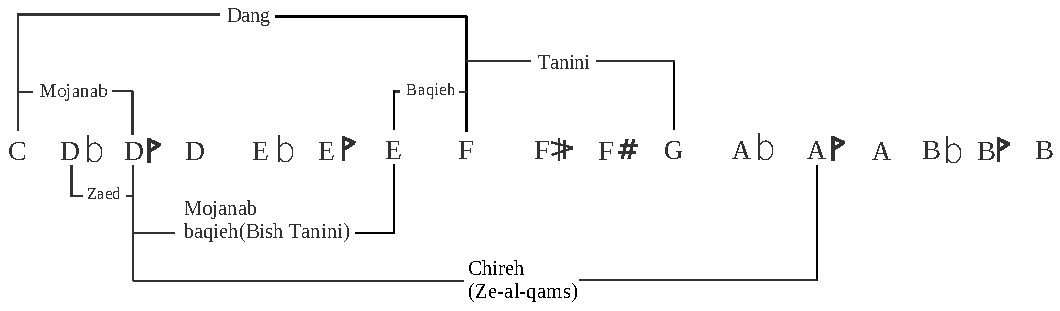
\includegraphics[width=0.95\linewidth]{figures/appendix_fig1_interval_names.pdf}
\caption{The 17 Iranian pitch classes spanning one octave, with a representative example
of each named interval (Zaed, Mojanab, Baqieh, Tanini, Bish-Tanini, Dang, and Chireh).}
\label{fig:appendix_intervals}
\end{figure}

\subsection*{Dang}
A Dang is a scale-like musical entity in Iranian classical music comprising four pitch
classes, in which the interval between the lowest and highest pitch class is a perfect
fourth. (The concept of Dang as used in performance practice carries additional dynamic and
contextual characteristics set aside here for simplicity.) Each Dang is built from a
specific ordered combination of three intervals, and each such combination carries its own
name. Dang-e-Shoor (Figure~\ref{fig:appendix_dang}) illustrates this structure.

\begin{figure}[htbp]
\centering
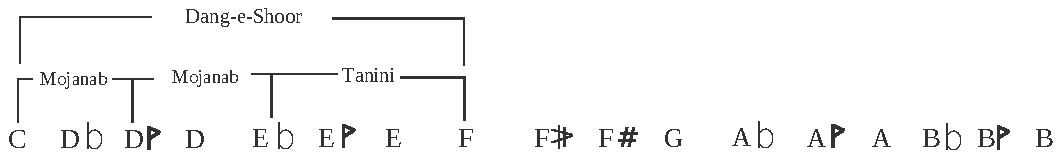
\includegraphics[width=0.95\linewidth]{figures/appendix_fig2_dang_e_shoor.pdf}
\caption{Dang-e-Shoor, a representative Dang, formed by the ordered interval combination
Mojanab--Mojanab--Tanini spanning a perfect fourth.}
\label{fig:appendix_dang}
\end{figure}

\subsection*{Tasks}
The two interval tasks classified 153 input patterns, representing every possible melodic
interval among the 17 Iranian pitch classes, into 24 output categories (interval types and
their inversions encoded separately) and 13 output categories (inversions collapsed),
respectively. The seven Dang tasks shared one classification logic but differed in how
dissonant Dangs were treated, as summarised in Appendix Table~1. Even-numbered Dang tasks
retained all 246 Dang patterns and collapsed progressively larger sets of dissonant Dangs
into a single dedicated dissonance category, while the odd-numbered member excluded those
Dangs from the training set. Task~1 applies no dissonance rule at all. Stimulus and category
counts for all eleven tasks are given in Table~\ref{tab:tasks}.

The three nested dissonance sets referenced in Table~\ref{tab:tasks} follow Mafi \cite{mafi2009} and are defined over the three successive intervals of a Dang as follows.

\begin{table}[htbp]
\centering
\caption{The nested dissonance sets used by Dang tasks 2--7. Each set contains the
previous one. Interval sizes are given in cents.}
\label{tab:dissonance}
\small
\begin{tabular}{@{}clp{0.52\textwidth}@{}}
\toprule
Set & Used by tasks & A Dang is treated as dissonant if it contains \\
\midrule
A & 2 (collapse), 3 (exclude) & a \emph{Zaed} interval (50) anywhere \\
B & 4 (collapse), 5 (exclude) & set A, or the adjacent sequence \emph{Baqieh--Baqieh}
(100, 100) or \emph{Baqieh--Mojanab} (100, 150) \\
C & 6 (collapse), 7 (exclude) & set B, or a \emph{Tanini+Baqieh} interval (300) anywhere,
or the adjacent sequence \emph{Mojanab--Baqieh} (150, 100) or \emph{Baqieh--BishTanini}
(100, 250) \\
\bottomrule
\end{tabular}
\end{table}

Applying these rules to the 246 enumerated Dangs yields the stimulus and category counts of
Table~\ref{tab:tasks}; the mapping is implemented exactly as stated in the deposited code
and is verified by the accompanying test suite.

\end{appendices}

\bibliography{references}

\end{document}
